\documentclass{article}

\usepackage[a4paper, hmargin=15mm]{geometry}
\usepackage[table]{xcolor}
\usepackage{tabularx}
\usepackage{fancyhdr}
\usepackage{lastpage}
\usepackage[colorlinks=true, linkcolor=black]{hyperref}
\usepackage{tikz}

\pagestyle{fancy}
\fancyhf{}
\fancyhead[L]{\hyperref[toc]{$\leftarrow$Indice}}
\fancyhead[R]{\thepage/\pageref{LastPage}}

\rowcolors{2}{gray!10}{white}

\newcommand{\riga}[2]{
	#1 & #2\\
}

\newcommand{\tabella}[2]{
	\addcontentsline{toc}{subsection}{Comandi #1}
	\begin{center}
		\begin{tabularx}{\textwidth}{|lX|}
			\hline
			\rowcolor{gray!20}
			\textbf{#1} & \textbf{Descrizione}\\
			\hline
			#2
			\hline
		\end{tabularx}
	\end{center}
}


\title{Programmazione ad'Oggetti}
\author{Leonardo Mengozzi}
\date{}
\begin{document}
	\maketitle

	\begin{center}
		\tiny Titoletti indice link a rispettive sezioni, in alto a sinistra "$\leftarrow$Indice" link a pagina Indice.
	\end{center}

	\tableofcontents\label{toc}

	\section{Approccio object-oriented}

	\section{Struttura Programma Java}
Un programma Java è composta da librerie di classi del JDK, Package\footnote{Contenitori, gerarcici tra loro, di una decina di classi di alto livello con scopo comune.} e Moduli\footnote{Insieme di Package costituente un frammento di codice autonomo.}, librerie di esterne e un insieme di classi fondamentali.

La classe cardine di un programma è la class main\footnote{Un main è il punto d'accesso di un programma.}.
\multiline{main}{}{CodiciEsempio/main.java}
Il parametro del main è un array di stringhe che sono i parametri che l'utente può immettere da tastiera quando il programma è lanciato da CLI. Poco usato.

\subsection{Esecuzione Programma}
\begin{enumerate}
	\item Salvare la classe in un file \textbf{"NomeClasse.java"}.
	\item Compilare con \textit{javac NomeFileClasse.java}. Genererà il \textbf{bytecode NomeFileClasse.class} per la JVM.
	\item Esegiure con \textit{java NomeFileClasse}. La JVM cercherà il main da cui partire a eseguire.
\end{enumerate}
Lavorando con più file: si compila tutto con \textit{javac *.java} poi si esegue solo il bytecode contenente la classe main.

\subsection{I package}
Per prassi nella cartella di un progetto, si fa corrispondere hai package auto-costruiti delle directory del file system.

Di default il package di una unità di compilazione\footnote{File.java compilabile atomicamente contenente classi una dopo l'altra.}, ".java", è la root di gerarchia.
Per definire il pakage di appartenenza si specifica a inizio sorgente:

\inline{package <pName>;}

Per poi usare una classe di un package bisogna importarla (non aggiunge codice nell'eseguibile):
\begin{itemize}
	\item \inline{import java...;} importa una singola classe.
	\item \inline{import java...*;} importa l'intero Package.
	\item \inline{import java.lang.*;} importazione di default.
\end{itemize}
Il nome completo di una classe dipende dal Package in cui si trova. Se non si importa bisogna specificare all'uso il nome completo.

\subsubsection{Compilazione ed'esecuzione Avanzata}
Per tenere sorgenti e eseguibili separati, in progetti grandi si dispone la cartella \textit{src} per i sorgenti (.java) e la cartella \textit{bin} per i bytecode (.class).

\oneline{javac -d "<dirExe>" [-cp "<lib1:|;...>"] <.../elencoSorgenti>}

\oneline{java -cp "<dirExe[lib1:|;...]>" <fullyClasseMain>}

\begin{itemize}
	\item \inline{-d} specifica al compilatore la cartella dove creare i .class. Se non già presente la crea.
	\item \inline{-cp} linka le classi dei percorsi specificati (divisi da : o ;) al classpath\footnote{Sottopercorso (insieme ordinato) di cartelle che corrisponde al percorso del package dichiarato per la classe corrispondente. Il classpath di default è il JRE (Java Runtime Environment).}.
	\item La JVM si aspetta il FQCN (Fully-Qualified Class Name).
\end{itemize}

\subsubsection{Gradle}
Build system ibrido composto da:
\begin{itemize}
	\item \textbf{Progetto} Cartella contenente i file \textit{build.gradle.kts} e/o \textit{settings.gradle.kts} (build files).
	\begin{enumerate}
		\item Il build contiene la logica di costruzione del software.

		\oneline{plugins\{java\}}

		Io creo \textit{src/main/java} per i .java e sarà creato \textit{build/classes/java/main} per i .class.
		\item Il settings contine la personalizzazione, come il nome del progetto.

		\oneline{rootProject.name="..."}
	\end{enumerate}
	\item \textbf{Plugin} Sofware contenente \textit{task} pronti all'uso, come per java.
	\item \textbf{Task} Singola operazione atomica del processo di costrutzione del software. Una esecuzione gradle richiede una o più task di cui sono automaticamente dedotte le dipendenze.

	Comandi: gradle tasks, gradle tasks --all, gradle compileJava, gradle clean.
\end{itemize}
L'esecuzione è delegata al compilatore del linguaggio specifico.

\textbf{Wrapper}: sofware scarica gradle e lo usa per creare il sofware.
File del wrapper: gradle/wrapper/gradle-wrapper.jar (wrapper in s'è), gradle/wrapper/gradle-wrapper.properties (versione), ./gradlew oppure gradlew.bat (eseguono il wrapper).

Per compilare:
\oneline{./gradlew compileJava}



\subsection{Convenzioni}
\begin{itemize}
	\item Linee max 90 caratteri e indenzazione 2-4 caratteri.
	\item Una sola istruzione per riga e quindi si definisce una sola variabile per riga, quando necessario, sempre inizializzata.
	\item Apertura "\{" a fine riga della dichiarazione e chiusura "\}" in linea a dove inizia la riga di apertura.
	\item Condice senza righe vuote di separazione a meno di metodi/costruttori.
	\item Non usare assegnamenti dentro espressioni e usare parentesi solo in espressioni non banali.
	\item Nomi classi e interfacce in "PascalCase". Nomi metodi, campi, variabili in "camelCase" e costanti in "SNAKE\_CASE". Nomi di package in minuscolo con numeri e senza "\_".
	\bigskip
	\item I metodi che returnano, senza parametri, si chiamano \inline{get...} oppure \inline{is/has...} se return boolean.
	\item I metodi che returnano void, e accettano parametri, si chiamano \inline{set...}.
\end{itemize}
	\subsubsection{I Commenti}
Oltre a \inline{//... e /*...*/} in java abbiamo \inline{/** ... */} un commento multi linea usato per generare documentazione.


\section{(Almost) Everything is an object}
Le variabili, contenitori con nomi, ora non denotano solo valori numerici (come in C), ma anche veri e propri oggetti irriducibili.

Non ci sono meccanismi per controllo diretto memoria. Le variabili sono nomi "locali" con riferimenti ad'\textit{oggetti} e non maschere di indirizzi in memoria a cui accedere direttamente.

Le variabili posso essere di tipo \textit{Java Types} quindi classi predefinite e autoimplementate oppure \textit{tipi primitivi}.

Visibilità legata al blocco di definizione.
Variabili non inizializzate sono inutilizzabili.

\subsection{Stack e Heap}
Gli oggetti sono memorizzati nell'\textbf{heap}. Tutte le variabili sono memorizzate nello \textbf{stack}.

Le variabili di tipo primitivo contengono direttamente il valore. Le variabili tipo classe contengono il riferimento dell'oggetto oppure null.

Nota: Uno stesso oggetto può essere puntato da variabili che si riferiscono alla stessa identità.

\subsection{Tipi Primitivi}
Ripasso: Un tipo classifica valori/oggetti tramite un nome, set valori, operatori.

I tipi atomici \textbf{signed} del C si sono mantenuti (non conveniva trattarli come oggetti) definendo un unica interpretazione:
\begin{center}
	\begin{tabular}{llll}
		\hline
		Tipi  primitivi & Dimensione & Minimo & Massimo \\
		\hline
		boolean & -- & -- & -- \\
		char & 16bits & Unicode 0 & Unicode $2^{16}-1$ \\
		byte & 8bits & -128 & +127 \\
		short & 16bits & $-2^{15}$ & $-2^{15}-1$ \\
		int & 32bits & $-2^{31}$& $+2^{31}-1$ \\
		long & 64bits  & $-2^{63}$& $-2^{63}-1$\\
		float & 32bits & IEEE754 & IEEE754 \\
		double & 64bits & IEEE754 & IEEE754 \\
		\hline
	\end{tabular}

	{\tiny Le librerie \textit{BigDecimal, BigInteger} gestiscono numeri di dimensione/precisione arbitraria.}
\end{center}

\textbf{typing statico}: espressioni tipo noto al compilatore, vantaggio intercettazione errori.

\textbf{Nota:} Uso memoria non dato a sapere al programmatore.

\subsubsection{Boolean}
Introdotto come tipo risultato delle espressioni e condizioni.
\begin{itemize}
	\item \textbf{Valori} true, false.
	\item \textbf{Operatori Unari} \inline{! (not)}. Peratori binari: \inline{\& (and), | (or), \^ (xor), \&\& (and-C), || (or-c)}\footnote{\inline{& e |} valutano sempre primo e secondo termine, essendo pensati per operazioni bit a bit mentre \inline{&& e ||} valotano il secondo operatore solo se necessario.}.
	\item \textbf{Operatori confronto numerici} \inline{<, >, <=, >=}.
	\item \textbf{Operatori di uguaglianza} \inline{==, !=}. Con gli oggett di base confronta i riferimenti.
	\item \textbf{Operatore ternario} \inline{<eb> ? e1 : e2}. restituisce e1 se eb è true, altrimenti restituisce e2. e1 e e2 espressioni dello stesso tipo.
\end{itemize}

\subsubsection{Caratteri}
Rappresentazione \inline{'carattere'} o \inline{'\u<0-65535>'}. Formato ASCII o UTF16 (16bit). I caratteri d'escape si fanno \inline{'\\<specificatore>'}.

\subsubsection{Interi}
\begin{itemize}
	\item \textbf{Codificati} in complemento a 2.
	\item \textbf{Operatori} \inline{+ ,-, *, /, \%, + e - unari, \&, |, ~, <<, >>, >>>}. Output stesso tipo Input.
	\item \textbf{Rappresentabili} in codifica decimale (1\_000\_000), ottale (0...), esadecimale (0x...).
	\item \textbf{Input tastiera} default int (più usato e efficente). Se voglio un long va aggiunta una "l" dopo il numero.
\end{itemize}

\subsubsection{Virgola mobile}
\begin{itemize}
	\item \textbf{Operatori} \inline{+ ,-, *, /, \%, + e -} unari.
	\item \textbf{Codificati} in IEEE754.
	\item \textbf{Rappresentabili} in codifica decimale o scientifica.
	\item \textbf{Input tastiera} default double. Se voglio un float (più efficente) va aggiunta una "f" dopo il numero.
\end{itemize}
\textbf{Ricorda}: IEEE754 ha errori di precisione che portano all'approssimazione dei risultati.

\subsection{Conversioni}
\begin{itemize}
	\item \textbf{Implicita} automaticamente applicata nelle esperessioni e nell'assegnamento portando tutti tipi a quello più "generale" presente nell'espressione. Detta \textit{coercizione}.

	$byte\to short \to int \to long \to float \to double$
	\item \textbf{Esplicito} fatto con operatore di casting: \inline{...=(<tipo>)<espressione>;}. Può causare perdità di informazioni.
\end{itemize}

\subsection{tipo statico e a rum-time}
\begin{itemize}
	\item \textbf{Tipo Statico}: Tipo di un espressione desumibile dal compilatore.
	\item \textbf{Tipo run-time}: Tipo effettivamente presente è tipo statico o sottotipo.
\end{itemize}

Per ispezionare il tipo a run-time:

\oneline{<espressione> instanceof <tipo>}

Restituisce \inline{boolean} e usato nella condizione di un \inline{if} permette di specializzare esecuzione.
\bigskip

\textbf{Downcast}: Creare nuovo riferimento di tipo statico all'espressione (da sovraTipo a sottoTipo):

\oneline{... (<tipoEffettio>)<espressione> ...}

\subsection{Autoboxing}
Ogni tipo primitivo può essere "boxed" in un oggetto.

\begin{itemize}
	\item \textbf{boxing} azione di inscatolamento di un tipo primitivo in un oggetto.
	\oneline{<Tipo> <variabile> = <Tipo>.valueOf(<tipoPrimitivo>)}
	\item \textbf{de-boxing} azione di estrarre un tipo primitivo da un ogetto.
	\oneline{... <varOggetto>.<tipoPrimitivo>Value() ...}
\end{itemize}

Boxing e De-boxing sono effettuati in automatico.

\subsection{Array}
Oggetti (variabili hanno riferimento nello heap) di lunghezza esplicita e acessibile, inacessibile fuori dai limiti (errore esecuzione), mutabili. Indirizzi elementi [0, lunghezza-1].

Sintassi:
\begin{itemize}
	\item \inline{<tipo>[] <nome> = new <tipo>[] \{v1,...,vn\};}
	\item \inline{<tipo>[] <nome> = new <tipo>[<dim>];}. Elementi inizializzati a valore default tipo (false, 0, null).
	\item \inline{<tipo>[] <nome> = \{v1,...,vn\};}
\end{itemize}

Note: Si possono fare array di array. Gli array di oggetti sono oggetti con puntatori ad'altri oggetti.

Accesso a variabile \inline{... <nome>[<ind>] ...}.

Per sapere la lunghezza dell'array \inline{<nome>.length}.

\subsubsection{Foreach}
Astazione \inline{for} in sola \textbf{lettura}, utile quando non importa ordine scorrimento elementi collezione e valore indice.

\oneline{for(final<tipo> <v>: <e>)}

\begin{itemize}
	\item \inline{v} è variabile del tipo indicato che vale via via ogni elemento della colezzione.
	\item \inline{e} è un espressione che restituisce una collezione di elementi del tipo indicato.
	\item Si può esplicitare \inline{final}, anche se non servirebbe, perchè il foreach crea una nuova variabile a ogni iterazione in realtà.
\end{itemize}
	\section{Classi}
Sono template (tipo, struttura in memoria, comportamento) per generare oggetti (istanza).

Le classi hanno un nome (NomeClasse) che sarà anche il nome del tipo per le variabili e del file.

I membri fondamentali di una classe sono:
\begin{itemize}
	\item \textbf{Campi}, descrivono la struttura/stato
	\item \textbf{Metodi}, descrivono i messaggi e il comportamento
\end{itemize}
Poi possiamo avere Costruttori, ecc.

Le classi sono tipi di dato in un linguaggio a oggetti tutto è un oggetto fino a un certo punto.

\multiline{strutturaclasse}{}{CodiciEsempio/StruturaClasse.java}

\subsection{Campi}
Sono lo stato attuale dell'oggetto. Nome con la minuscola.
Simili hai membri di una struttura C, con la differenza che possono essere 0,1,diversi (5-7max). Simili a variabili (tipo+nome), ma non si può usare \textit{var}.
Possono essere valori primitivi o altri oggetti (anche della classe stessa).
L'ordine dei non conta.

I campi sono iniziabili alla dichiarazione dell'oggetto (coi parametri), sennò sono inizializzati in base al tipo a \textbf{0, false, null}. Mai alla dichiarazione si inizalizzano (...=...;).

\oneline{public|private|"" [final] <tipo> <nomeCampo>;}

Uso dei campi lato utente: Assegnamento \inline{... obj.campo = ...}, Lettura \inline{... = obj.campo ...}

\subsection{final e costanti}
Modificatore (da usare quando si può) per campi, variabili e parametri. Dopo inizializzazione non più modificabile il valore.

Per variabili di tipo classe non si può cambiare il riferimento all'oggetto, ma i campi dell'oggetto si.

\oneline{<tipo> final <nomeVar [= new ... | valore;]}

Per fare le \textbf{costanti} (NOME\_COSTANTE) usare \inline{static final ...;}. Soluzione a \textit{Magic Number}.

\subsubsection{Oggetti immutabili}
Oggetti i cui campi non si modificheranno mai, dopo la prima modifica del costruttore.

Si creano dichiarando \inline{final private} tutti i campi della classe di tipo: tipi primitivi o oggetti immutabili.

\subsection{Metodi}
Definiscono il comportamento dell'oggetto. Nome con la minuscola.
Simili a funzioni C. Hanno un intestazione (tipo di ritorno|void, nome, argomenti) e un corpo.
I metodi di una classe possono essere 0, 1, diversi.

i metodi possono leggere/scrivere i campi.

Uso dei metodi lato utente \inline{... obj.metodo() ...}. L'invocazione del metodo, corrisponde a inviare un messaggio al receiver (obj nell'esempio) azionando l'esecuzione del corpo del metodo.

\multiline{strutturametodo}{}{CodiciEsempio/StrutturaMetodo.java}

Nota: Classi POJO sono classi con solo campi privati, costruttori e metodi get e set.

\subsubsection{Variable arguments}
Per passare un numero indefinito di parametri di un certo tipo:

\oneline{<tipo> <nomeMetodo>([<parametri>], <tipo>... <nomeParametro>) \{...\}}
\begin{itemize}
	\item Va definito come ultimo o unico parametro.
	\item Nel corpo del metodo sarà trattato come un array di \inline{<tipo>}.
	\item Il chiamante passa al metodo una lista di parametri di \inline{<tipo>}.
\end{itemize}

\subsubsection{return this}
Un metodo può ritorna \inline{this}, l'oggetto corrente. Deve avere come tipo di ritorno la classe stessa.

Usato per concatenare più metodi in una sola espressione, combinando i risultati parziali, e restituendo con l'ultimo metodo l'oggetto processato:

\inline{... obj.m1().m2()...mThis();}

Questo schema è detto \textbf{fluente}.

\subsection{Costruttore}
Simile a un metodo con nome il nome della classe, senza tipo di ritorno e opzionalmente dei parametri formali.

\inline{NomeClasse([parametri]) {...}}

Se non si definisce il costruttore viene implicitamente inserito il costruttore di default (0 parametri) che inizializza i campi ai tipi di default.

Nota: per fare una classe non istanziabile basta fare i costruttori \inline{private/protected}.
\subsubsection{Overloading}
Si possono definire più costruttori e metodi, ma non è una buona pratica.
Nel caso devono essere \textbf{distinguibili dal numero e/o tipo} dei parametri.

I costruttori si possono \textbf{invocare a vicenda} (riuso codice). \inline{this(...)} deve essere la prima riga del corpo del costruttore.

\multiline{riusocostruttori}{}{CodiciEsempio/RiusoCostruttori.java}

\subsection{this}
Variabile contenente il riferimento all'oggetto che sta gestendo il messaggio corrente. Si usa per rendere meno ambiguo il codice accedento tramite \textit{this} a campi o metodi. (Usare sempre).
\inline{... this.cmapo ... this.metodo() ...}

\subsection{static}
Scollega metodi e campi dagli oggetti di una stessa classe, rendendoli condivisi tra essi. I metodi diventano funzioni pure e i campi variabili globali alla classe.

Si possono fare classi solo statiche (utility class, NomeClasse+s) più non statiche (approccio migliore) o miste (campi e metodi static in fondo).

Richiamo fuori dalla classe: \inline{... nomeClase.campo|metodo() ...}.
Richiamo nella classe come normale campo o metodo.
Richiamabile anche da un oggetto.

\oneline{static campo|metodo|classe}

Quando \inline{static}?
Si fanno statici i metodi o campi che sono indipendenti dallo stato di un oggetto della classe. Fanno un servizio indipendente dal singolo oggetto.

\subsection{Livelli d'accesso}
Si antepongono a classi, metodi, campi, costruttori per definire il grado di utilizzo, in ordine crescente di libertà:
\begin{enumerate}
	\item \inline{private} Visibile e richiamabile solo nella classe di definizione.
	\item \inline{package} default (no keyword). Visibile e richiamabili dentro il package e invisibili fuori.
	\item \inline{protected} Visibile alla classe corrente e dalle sotto classi ricorsivamente. (in java anche al package).
	\item \inline{public} Visibile e richiamabile da qualunque classe.
\end{enumerate}

In una unità di compilazione una sola classe è \inline{public} e con lo stesso nome del file.

Vantaggio: Si può far rispettare al meglio il contratto\footnote{Insieme degli scienari d'utilizzo e quindi aspettative di un utente al suo utilizzo.} di un oggetto.

\subsubsection{Incapsulamento}
\begin{center}
	Scopo: Avere controllo su come vengono usati i dati.
\end{center}

\colTwo{Dichiaro \inline{public} solo metodi/costruttori, di "design", necessari all'utente per interagire/creare l'istanza della classe.}{Dichiaro \inline{private} tutti i metodi/costruttori di "implementazione", e \textbf{tutti i campi}.}{45}{45}

Cosi modifiche implementative non influenzano uso dell'utente. Controllo dati e riuduco possibilità errori lato utente. Maggior distacco tra dato e implementazione. (\textit{Information hidding} = nascondere implementazione informazioni).

\bigskip

\textbf{Principio di decomposizione (\textit{divide et impera})}: Soluzione di un problema complesso è la somma di due o più sotto problemi più semplici, tra loro indipendenti.

Tali sotto problemi devono avere il minor numero di dipendenze\footnote{Riferito alle classi è quando una classe usa al suo interno un'altra. Ciò può comportare modifiche a cascata rischiando la \textit{sindrome dell'"intoccambilità"}.} reciproche. Permettendo maggior autonomia, più modifiche senza danni collaterali e meno interazioni.

Una buona divisione da moduli con basse dipendenze esterne e alte dipendenze interne.

Nella OO le suddivisioni base sono pacakge, classi e metodi.

Nota: Per rispettare l'incapsulamento quando si fa un get di un tipo non primitivo, bisogna restituire una copia del campo e non il campo stesso.

\subsection{Precisazioni}
Inizializzazioni particolari degli oggetti Stringa:
\begin{enumerate}
	\item \inline{... = new String();}, stringa vuota (è diverso da null).
	\item \inline{... = "..."}, come in C, comportamento speciale degli oggetti Stringa.
\end{enumerate}

\subsection{Fasi Implementazione}
\begin{enumerate}
	\item Progettazione della parte pubblica della classe (nome classe, signatura metodi e costruttori necesari).
	\item Costruzione dello stato (campi privati, con nome diverso dai metodi relativi).
	\item Completamento implementazione. (test).
	\item Miglioramento codice finale (commenti, eliminare \textit{Magic Number}, fattorizzare sotto-funzioni). (test).
	\item Test del risultato con test-case. (test-driven development con JUnit).
\end{enumerate}

\section{Oggetti lato Utente}
Dichiarazione, creazione, inizializzazione:

\inline{<Tipo | var> <nome> = <new Tipo([argomenti]) | altraVariabile | null>;}
\begin{itemize}
	\item \inline{<Tipo> <nome>;} Si può solo dichiarare una variabile oggetto per poi crearla e inizializzarla successivamente.
	\item solo quando si scrive \inline{new} (Keyword di linguaggio di chiamata al costruttore) si crea e inizializza un oggetto dalla classe indicata. \inline{new} da il riferimento (\inline{this}) dell'oggetto alla variabile.
	\item \inline{var}\footnote{Local variable type inference.} fa infierire\footnote{Far dedurre al compilatore il tipo della variabile locale dall'espressione assegnata.} il tipo della variabile locale per allegerire il codice. Se manca l'espressione non va, esempio \inline{var i;}.
	\item \inline{altraVariabile} deve essere della stessa classe della variabile che sto definendo.
\end{itemize}
	\section{Dipendenze}
Il minimo numero di dipendenze fra classi sono manifestazione di "riuso" di codice e ne fanno un sistema e non un mero gruppo.

I tipi di dipendenze sono:
\begin{itemize}
	\item \textbf{Associazione} (uses),  un oggetto ne usa un altro.
	\item \textbf{Composizione} (has-a), un oggetto ne aggrega altri.

	Un oggetto di una classe \textit{si compone di} (campi) un insieme di altri oggetti, di altre classi.

	Tale composizione può essere permanente (campo final) o opzionale (campo possibilmente \inline{null}), multipla nota (più campi) o sconosciuta (campo array).
	\item \textbf{Specializzazione} (is-a), una classe ne specializza un'altra.
\end{itemize}

Nota: Nella composizione alla cancellazione dell'oggetto utilizzatore gli oggetti usati vengono cancellati a loro volta. Diversamente nell'aggregazione questi persistono.




\subsection{Poliformismo Inclusivo (subtyping)}
Fornire sovratipi che raccolgono classi uniformi tra loro.
Gode del principio di sostituibilità utile a creare collezioni omogene.

\textbf{Upcast}: Per il principio di sostituibilità quando ci si aspetta A si può usare B ma solo con le cose di A e non quelle esclusive di B. Ciò perchè B risponde almeno a tutti i messaggi di A (hanno i medesimi contratti).
\medskip

\textbf{Con Interfacce}
Sia B classe sottotipo di A interfaccia, con medesimi metodi (contratto) e altro possibilmente. Facile far aderire una classe a un iterfaccia.
\medskip

\textbf{Con Classi}
Sia B sottotipo di A, con medesimi metodi e campi (contratto+comportamento) e altro possibilmente. B e A hanno un comportamente compatibile.

\textbf{In memoria}: Intestazione (16byte) con indicazioni a run-time sulla classe dell'oggetto, tabella puntatori per vtable, campi privati di Object. Poi campi classe partendo da quelli della super classe.
\bigskip

\textbf{Poliformismo Parametrico} (genericità): ???.




\subsection{Interfacce}
Sopra tipo con caratteristiche comuni. Le classi implementative sono sotto tipi dell'interfaccia.

\bigskip

Separa esplicitamente l'interfaccia (contratto, fisso) dalla realizzazione (implementazione, variabile) della classe.

Consente diverse realizzazioni di un contratto, usabili omogeneamente. (più classi implementano medesime funzioni e si vuole usarele come fossero la stessa).

\oneline{interface <NomeInterfaccia> \{...\}}

\begin{itemize}
	\item Nuovo tipo solo dichiarabile (no \inline{new NomeInterfaccia()}) con valore oggetti delle classi che implementano l'interfaccia.

	\textbf{Principio sostituibilità di Liskov}: A sottotipo di B, ogni oggetto A deve essere usabile dove ci si attende un oggetto B.
	\item Un oggetto tipo interfaccia consente solo chiamate ai metodi definiti dall'interfaccia e esegue l'implementazione specifica classe implementativa dell'interfaccia.

	\oneline{<NomeInterfaccia> <nomeVar> = new <ClasseImplementativa>();}

	Tipo statico è interfaccia e tipo run-time è tipo classe implementativa.
	\textbf{Late binding}: Codice da eseguire scelto dinamicamente, dipende da classe implementativa dell'interfaccia tipo della variabile.

	\item Include solo intestazioni di metodi. Sono automaticamente \inline{public} e non si specifica.
	\item Compilato come una classe (produce un .class).

	\item Un interfaccia può estendere altre interfacce.

	\oneline{interface <NomeInterfaccia> extends int1[,...] \{...\}}

	Nel corpo dell'interfaccia si specificano solo i metodi che aggiunge.
\end{itemize}

\oneline{class <NomeClasse> implements <NomeInterfaccia[,...]> \{...\}}

\textbf{Una classe può implementare più interfacce.}

\begin{itemize}
	\item Deve implementare il corpo di tutte le intetazioni di metodo delle interfacce (metodi in comune implementati una volta). La classe potrà avere altri metodi suoi.
	\item Le istanze avranno tipo la classe e le interfacce.
\end{itemize}

Nota: L'interfaccia è il sopra tipo/insieme delle classi, è più generale, ma fornisce meno funzionalità.

Nota: La classe che rispeccia l'interfaccia si chiama \textit{impNnomeInterfaccia}.




\subsection{Composizione/delegazione}
Data una classe (di cui possono non avere i sorgenti) ne realizzo un'altra con caratteristiche solo in parte diverse, ovvero una specializzazione. Questa nuova classe potrebbe sostituire la precedente (gerarchia \textit{is-a}).

Senzia violare \textbf{DRY}: Don't Repeat Yoursealf.

Nella nuova classe:
\begin{enumerate}
	\item \textbf{Incapsulare} un oggetto della classe da modificare/estendere mediante campo \inline{private final}\footnote{Cosi che l'oggetto una volta inizializzato non possa essere cambiato ma si possa allo stesso tempo adoperare metodi e campi di conseguenza.}. Sarà inizializzato nel costruttore della nuova classe.

	\item \textbf{Metodi} possono delegare all'oggetto incapsulato e essere di più o meno, ampliando cos'ì le funzionalità. Viola poco DRY.

	\item \textbf{Combinare} con l'uso delle interfacce per ottenere la sostituibilità.
\end{enumerate}
Quando si può è meglio usare i metodi "ridefiniti" che "originali" per rispettare l'incapsulamento.




\subsection{Ereditarietà}
Definisce una classse specializzandone una esistente \textbf{ereditando}. Rispetta DRY.

\oneline{class <ClasseFiglio> extends <ClassePare> \{...\}}

\textbf{Ereditarietà singola (tree), una classe può estenderne solo un'altra.}

\begin{itemize}
	\item Eredita (usabili) campi, metodi, costruttori non \inline{private}.

	\item Costruttori non privati del padre richiamti solo da costruttori figlio (c.Figlio>=c.Padre), per inizializzare campi Padre.

	\oneline{super(<parametri>)}

	Se precesente deve essere la prima riga dei costruttori del figlio che devono avere almeno i parametri dei costruttori del padre.

	Costruttori default padre chiamato se \inline{super()} assente/posizione errata.

	\item Figlio può aggiungere campi e metodi propri a quelli del pare (m.Figlio>=m.Padre) essendone una specializzazione.

	\item Figlio acede a campi Padre (\inline{private}) con get/set \inline{protected} per rispettare incapsulamento.

	\item Classe Figlio vede la "catena" di ereditarietà come un unica sovra classe da cui eredità.

	\item Una classe col modificatore \inline{final} non è ereditabile.
\end{itemize}

Nota: Bastano i binari per estendre una clsse.

Come le interfacce anche l'ereditarietà gode della sostituibilità. Posso fare variabili di tipo Padre ma che referenziano oggetti tipo Figlio. Questo perchè i Figli essondo delle specializzazioni "sono anche padre".

\subsubsection{Overriding}
Riscrizione di uno o più metodi \inline{public} del Padre nel Figlio.

\begin{itemize}
	\item Per sovrascrivere un metodo bisogna usare la stessa firma, a meno che del modificatore d'accesso che può solo aprirsi verso uno meno ristrettivo (fino a public).

	\item Un metodo definito col modificatore \inline{final} non è Overridabile.

	\item Il metodo riscritto può invocare la versione Padre con \inline{super.<metodoPadre()>}. Usabile non solo in caso di overdding.

	\item Un metodo ereditato o sovrascritto che usa \inline{this} chiamerà la versione del metodo della classe chiamante (come ogni metodo).

	\item I metodi override hanno opzionalmente la notazione \inline{@Override} utile al programmatore e al compilatore per controlli di sintassi.
\end{itemize}

\subsubsection{Vtable}
Nomi: vtable, call table, dispatch table.

Riporta la classe con il body da associare a ogni metodo definito o ereditato di una classe.

\textbf{Nella Memoria}: Nello stack abbiamo le variabili che fanno riferimento a oggetti di una certa classe, memorizzati nella heap. Dentro la memoria di questi oggetti nella heap si hanno i riferimenti alle vtable definite per ogni classe. Queste tabelle per ogni metodo della classe dicono se usare la versione della classe corrente (metodo ex-novo o sovrascritto) oppure di una sovraclasse.

\subsubsection{Classe Object}
Una classe estende sempre indirettamente la classe \inline{Object}.
\inline{Object} è la radice di ogni gerarchia d'ereditarietà.

Fornisce metodi di uso generico:
\begin{itemize}
	\item \textbf{toString()} Restituisce una rappresentazione in stringa dell'oggetto (utile per il debug).Automaticamente chiamato dall'operatore "+" nelle concatenazioni tra stringhe e oggetti.
	Ogni classe deve sovrascriverlo.
\end{itemize}

\textbf{Vantaggio?} Fattorizza comportamento comune e crea funzionalità che lavorano su qualunque oggetto.




\subsection{Classi Astratte}
Classi dal comportamento parziale, fatte per raggruppare contratti+comportamenti comuni e opzionalmente contratti successivamente specializzati.

\oneline{abstract class ...}

\begin{itemize}
	\item Fornisce codice comune a classi figlie che la specializzano.
	\item Metodi già implementati, spesso \inline{final}, definiscono il comportamento comune.

	Metodi \textit{astratti}, opzionali, hanno solo il contratto. Le classi figlio ne definiranno il comportamento specifico. Vanno definiti \inline{abstract}:
	\oneline{abstract <tipo> <nomeMetodo>([<parametri>]);}
	Metodi astratti si definiscono solo in classi astratte.

	\item Possono contenere campi, costruttori.

	\item Classi non istanziabili (no \inline{new}).
	\item Una classe astratta può specializzare un'altra classe astratta o un interfaccia senza l'obbligo di specializzarne i metodi.
	\item Una classe astratta può estendere una classe non astratta.
	\item Una classe non astratta è tenuta a specializzare i metodi astratti della classe astratta da cui eredità.
\end{itemize}Intermedio tra ereditarietà tra classi e interfacce.


	\section{OOP2.0}
Nella OOP1.0 abbiamo il riuso per composizione, estensione, poliformismo inclusivo (subtyping).

La OOP2.0 aggiunge il poliformismo parametrico (generics), ???, con lo scopo di dare maggiore controllo al programmatore e espressività al linguaggio JAVA.

\begin{center}
	\begin{tikzcd}
		{[.java]} \arrow[rr, "Compilatore"] \arrow[rr, "JavaNew \to JavaVintage"', dotted, bend right] &  & {[.class]} \arrow[rr, "JVM"] &  & {[.exe]}
	\end{tikzcd}
\end{center}

Il compilatore risolve i costrutti della OOP2.0 trasformandoli in costrutti della OOP1.0 lasciando la JVM invariata.

\subsection{Generics}
\colTwo{\textbf{Scopo}: Creare funzionalità di lavorare uniformemente su oggetti indipendentemente dal loro tipo che diventa un parametro della funzionalità.}{\textbf{Vantaggio}: Fattorizzare, tramite astrazione, soluzioni/classi ricorrenti altamente simili in una unica soluzione/classe riusabile.}{45}{45}

Concetti chiave:
\begin{itemize}
	\item La \textbf{type-variable}, solitamente "X", è una variabile che contiene il tipo dell'oggetto a run-time.
	\item La type-variable è usabile ogni qualvolta si potrebbe scrivere un tipo.
	\item Possono esserci più type-variable.
	\item Tipi primiti non accettati, usare i Wrapper automaticamente risolti dall'autoboxing.
	\item Non passare tutti type-variabile lato utente è errrore.
\end{itemize}

\multiline{}{}{CodiciEsempio/Generici.java}
\textbf{Inferenza dei parametri}: Nella \inline{new} i type-variabile si omettono lasciando il \textit{diamond symbol} "$<>$". Alternativa usare la \inline{var}. In rari casi entrambi.

\textbf{Non posso} fare array di generics in una classe generics, vanno fatti di \inline{object} con i dovuti cast.

\bigskip

Per creare contratti uniformi si fanno interfacce generiche:

\oneline{... interface <nomeInterfaccia><X [, Y, ...] \{...\}}

Le type-variable sono usate nei metodi defini e le classi implementative le deve istanziare.

\bigskip

Metodi che lavorano e restituiscono qualsiasi tipo:

\oneline{def:... <X [, Y, ...]> <tipoRitorno> <nomeMetodo>(<parametri>) \{...\}}

\oneline{call:... <X, [Y, ...]><nomeMetodo>(<parametri>)...}

Inferiti automatica alla chiamata (non serve diamond symbol).

\bigskip

\textbf{Implementazione}: Il compilatore, in fase \textit{erasure}, sostituisce i generics usando il subtyping con object e facendo upcast implicito nelle classi che diventano monomorfiche, mentre lato utente usa autoboxing e downcast esplicito.

\subsection{Wildcards}
Tipi che permettono di esprimere un insieme di tipi accettati per un parametro, che usa generics, di metodo.

\oneline{<tipo> <nomeMetodo>(Tipo<? extends | super tipoRiferimento> nome,...) \{...\}}

Solo \inline{?} indica qualsiasi type-variabile. Vantaggio da un codice leggero.

\subsection{Classi innestate}

\subsection{Lambda expression}

	\section{UML (Class Diagram)}
Linguaggio grafico, OO-based, di modellazione di software.
\begin{itemize}
	\item \textbf{Rettangoli}: un box rettangolare per classe o interfaccia diviso in:
	\begin{enumerate}
		\item Nome classe. Nel caso delle interfacce aggiunge \inline{<<interface>>} a sinistra del nome.
		\item Campi (solo per classi). Signatura: \inline{nome : tipo}.
		\item Metodi e costruttori. Signatura: \inline{nome(arg1:tipo,...):tipoRitorno}.
		Se \inline{final} si indica l'attributo \{leaf\}
	\end{enumerate}
	- indica \inline{private}, + indica \inline{public}, \# indica \inline{protected} e sottolineato indica \inline{static}.

	Metodi e classi astratte si scrivono in corsivo.
	\item Dipendenze tra classi:
	\begin{itemize}
		\item Composizione è arco con rombo.
		\item Associazione è arco con freccia.
		\item Generalizzazione è arco tratteggiato con triangolo vuoto, raggruppabile.
		\item Estensione è arco con triangolo pieno, raggruppabile.

		Nella classe figlia si specificano solo le aggiunte e ovveride.
	\end{itemize}
	L'arco può essere indicato con le molteplicità: 1,0, n, 0...1, 1...n.

	\item Spesso accompagnato da descrizione testuale.
\end{itemize}

Spesso si omette tutto ciò che non è "design" e le signature ed'alcune relazioni.

	\section{Design Pattern}
Approccio fondamentale:

\begin{center}
	\begin{tikzcd}
		Interfacce               &  & {} \arrow[ll, "concetto"', no head, maps to] \\
		ClassiAstratte \arrow[u] &  & {} \arrow[ll, "condiceComune"', no head, maps to]              \\
		ClassiConcrete \arrow[u] &  & {} \arrow[ll, "implementazioni"', no head, maps to]
	\end{tikzcd}
\end{center}

Variabili, argomenti, tipi di ritorno sono interfacce mentre le \inline{new} sono solo di classi Concerete.

\begin{itemize}
	\item \textbf{Iteratore (Iterator)}: Oggetto usato per accedere ad'una sequenza d'elementi (presi da una sorgente di dati).
	\multiline{}{}{CodiciEsempio/iterator.java}


\end{itemize}

	\section{Collezioni}
Il Java Collections Framework (JCF), parte del \inline{package java.util}, gestisce strutture dati e relativi algoritmi.
\begin{figure}[h]
	\centering
	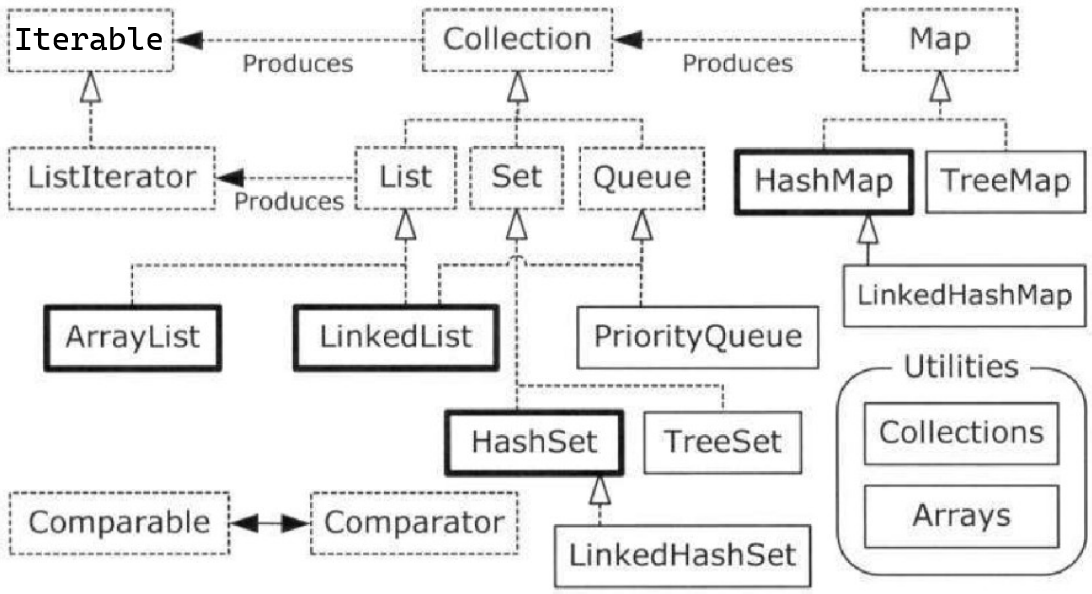
\includegraphics[width=0.8\textwidth]{JCF.png}
\end{figure}

Di nostro interesse sono:
\begin{itemize}
	\item Interfacce: Collection, List, Set, Iterator, Comparable.
	\item Classi: ArrayList, LinkedList, HashSet, HashMap.
	\item Classi Funzionalità: Collections, Arrays.
\end{itemize}

Fondamentalmente ci vengono fornite le collezioni (List, Set, Queue) e Map.

Tutti con un generic.

map: funzioni che metoono in relazione elementi di due gruppi.

in java le collezioni sono tutte mutabili, ovvero si possono modificare gli elementi.

tutte hanno add e toString().

\subsection{Iterable e Iterator}
\colTwo{Una classe che implementa l'interfaccia \textbf{\inline{Iterable<X>}} può essere iterata.}{Una classe di supporto che implementa l'interfaccia \textbf{\inline{Iterator<X>}} dice come essere iterata.}{45}{45}

\multiline{}{}{CodiciEsempio/Iterable.java}

Le due classi usate insieme possono iterare collezioni.

Esempio d'uso è nel foreach, che conosce le due interfacce, è può iterare qualunque oggetto di una classe che implementa \inline{Iterable<X>} e che usa un oggetto di una classe che implementa \inline{Iterator<T>}.

\subsection{Collection}
Interfaccia radice gerarchia interfacce di collezione (gruppi oggetti), estende \inline{Iterable}, e definisce:
\begin{itemize}
	\item Un costruttore vuoto. Assunto implicito.
	\item Un costruttore che accetta una Collection per l'inizializzazione. Assunto implicito.
	\item Operazioni di modifica opzionali.
	\item Operazioni di ricerca basete su Object.equals().
\end{itemize}

\multiline{}{}{CodiciEsempio/Collectoce.java}

I metodi \inline{contains e remove} applica il metodo \inline{Object.equals()} all'oggetto passato con tutti gli elementi della collezione.
Come argomento accetta \inline{Object} per poter confrontare oggetti anche non della stessa classe (potenzialmente uguali per le regole di confronto).

\subsubsection{Collezioni immutabili}
L'unico modo per creare una collezione di valori non modificabili ma solo leggibili.

\oneline{final ... = Set.of| copyOf(...);}
\oneline{final ... = List.of|  copyOf(...);}


\inline{Set | List.of| copyOf()} permette che i valori non siano cambianti e \inline{final} fa si che la variabile non sia riassegnata, rendendo il tutto un blocco unico.

\subsection{List}
Collezione estendibili sequenzializzata con indice. Aggiunge metodi per accesso elementi secondo posizione (O-based). Sono permesse ripetizioni di elementi (anche null).

Estende l'interfaccia \inline{ListIterator<E>} che estende \inline{Iterator<T>} permettendo di scorrere gli elementi sia "in avanti" che "in dietro".

\medskip

Nota: Scandire quando possibile elemnti via iteratore e non indici.

\medskip

Implementazioni sono ArrayList (O(1) tranne add O(n) ammortizzato), con \inline{trimToSize()| ensureCapacity()}, e LinkedList che implementa l'interfaccia Queue (FIFO o LIFO) e Deque.

\subsection{Set}
Collezione estendibili senza ordine e duplicati (\inline{Object.equals()} sempre \inline{false} e al massimo un \inline{null}). Non aggiunge metodi a Collection.

Per migliorare le prestazioni di \inline{contains()} si usa l'approccio \textbf{HashSet (O(1) aromtizzato)} che lega oggetto e posizione, o \textbf{TreeSet (O(logn))}.

Nota: I costruttori di HashSet accettano la dimensione iniziale stimata e un fattore di crescità, se basso hashing veloce, se alto hashing risparmia memoria.

\subsubsection{Ordinamento}
Per rendere gli oggetti di una classe ordinabili possiamo definire il criterio d'ordinamento:
\begin{itemize}
	\item \textbf{Interno} alla classe tramite l'implementazione dell'interfaccia \inline{Comparable<T>}.
	\multiline{}{}{CodiciEsempio/Comparable.java}

	Permette di comparare due oggetti dello stesso tipo secondo un unico criterio.

	\oneline{obj1.compareTo(obj2);}

	\item \textbf{Esterno} alla classe tramite una classe comparatore che implementa l'interfaccia \inline{Comparator<T>}.
	\multiline{}{}{CodiciEsempio/Comparator.java}

	Permette di comparare due oggetti dello stesso tipo secondo tanti criteri quante sono le classi comparatore.

	\oneline{objComparator.compare(obj1, obj2);}
\end{itemize}

Sia \inline{compareTo} che \inline{compare} restituiscono 0 se i due oggetti sono guali, un numero positivo se this o o1 è maggiore oppure un numero negativo se this o o1 è minore.

TreeSet e tante altre classi sfruttano l'ordinamento tra gli oggetti.

\subsection{Moduli}
Le classi statiche Array e Collections forniscono funzioni di base.

Array ha varie versioni di metodi per supportare tutti i tipi mentre Collections ne ha una per tutti.

\subsection{Map}
Collezioen estendibile di funzioni che mappano  Key in Value.

\oneline{public interface Map<K,V> {...}}

Map è biunivoca, due Value diversi non possono avere la stessas Key.

Implementazioni: HashMap, TreeMap.

\subsubsection{Map.Entry}
La mappa, internamente, ha un Set di Entry (coppie chiave-valore). Entry è una StaticNested \inline{interface}.

\multiline{}{}{CodiciEsempio/map.java}

Quindi per iterare una mappa si usa $entrySet()$ e il tipo degli elementi è $Map.Entryz<K, V>$.
	\section{Git}
Git è un sistema di controllo di versione (SCV).

Un SCV può essere \textbf{distribuito}, ovvero ogni svilupparore localcomente ha una copia dell'intero "progetto" (repository), oppure \textbf{Centralizzato}, ovvero gli sviluppatori lavorano in sottoparti di un'unico progetto in remoto.

Git usa il modello distribuito per la maggiore scalabilità e facilità di branching e merging.

\subsection{Concetti}
\begin{itemize}
	\item \textbf{Repository}: Contiene l'interastoria del progetto tramite l'uso di meta dati contenuti in una cartella nascosta della root directory.

	La struttura di una repository git è un alberlo/grafo.

	\item \textbf{WorkTree/WorkingDirectory}: Insieme di file della root directory che costituiscono il progetto. Sono esclusi i meta dati.

	\item \textbf{Staging}: Stato, o contenitore, in cui metti le modifiche dei file del workTree che voglio salvare col prossimo commit. Dopo un commit lo staging è vuoto.

	\item \textbf{Commit}: Stato salvato del progetto tramite tracciamento differenziale\footnote{Raccoglie le modifiche neccessarie a trasformare il commit precedente in quello attuale.}. Inoltre crea uno \textit{snapshotting} dello stato del workTree.

	Meta dati di un commit: commit padre (assente=commit iniziale, multiplo=commit di fusione), autore, messaggio, id univoco.

	\item \textbf{Branch}: Sequenza di commit con un nome. Usato nome di default al primo commit se non è stato indicato.
\end{itemize}

\subsection{Riferimenti ai commit}
I riferimenti ai commit sono chiamati \textit{tree-ish} e sono validi il nome del commit, il suo id (full o short), il nome del branch che fa riferimento all'ultimo commit avvenuto su quel branch, e HEAD.

HEAD è un nome speciale di commit che si riferisce al commit corrente ed'è linkata al branch del commit. Essenziale per muoversi nel workTree.

\begin{itemize}
	\item \textbf{Riferimento assoluto}: Esplicito il tree-ish a cuoi voglio spostare la HEAD.

	\item \textbf{Riferimento relativo}: Si fa \inline{tree-ish~i} per dire l'i-esimo commit padre del tree-ish in cui voglio spostare la HEAD. In caso di merge seleziona il primo.
\end{itemize}

A ogni nuovo commit la HEAD vi ci si sposta automaticamente.

\subsection{Operazioni base}
\begin{itemize}
	\item \textbf{Configurazione Globale}: Configura git a livello di sistema.

	\oneline{git config --global category.option value}

	\item \textbf{Configurazione Repository}: La configurazione di repository corrente sovrascrive quella globale.

	\oneline{git config category.option value}

	\item \textbf{Inizializzazione Repository}: Inizializza una repository nella directory corrente tramite il .git che esplicità la root directory.

	\oneline{git init}

	Eliminare il .git comporta l'eliminazione della repository locale.

	\item \textbf{Staging}: Per aggiungere allo staging:

	\oneline{git add <files>}

	Aggiungere allo staging un file che non esiste più è l'equivalente della sua eliminazione nel prossimo commit.

	Aggiungere allo staginig un file che ha lo stesso contenuto di un file che non esiste più è l'equivalente della sua rinominazione.

	Per rimuovere dallo staging:

	\oneline{git reset <files>}

	\item \textbf{Commit}: Fa il salvataggio in un nuovo commit dei file selezionati nello staging. Data e id autogenerati.
	La HEAD deve essere sull'ultimo commit di un branch.

	\oneline{git commit -m "..."}

	Richiede la configurazione del nome e email dell'autore e del nome del branch.
	Cose da scrivere in un messaggio: file eliminati, aggiunte, modifiche.

	\item \textbf{Stato della repository}: Mostra informazioni sul branch corrente, quali file sono modificati, lo stato dello staiging:

	\oneline{git status}

	\item \textbf{Checkout}: Sposta la HEAD nel tree-ish specificato, se non ci sono modifiche volatili, aggiornando i file alla versione del tree-ish specifiato.

	\oneline{checkout <tree-ish>}

	Fatto checkout si è in modalità \textit{detached head} (HEAD delinkata dal branch) e i commit fatti saranno persi fino.

	\item \textbf{Estrazione di file}: Altra funzione di checkout che permette di estrarre (riprisinare lo stato nella HEAD) da un tree-ish i file indicati.

	\oneline{git checkout <tree-ish> -- file1 [file1 ...]}

	\item \textbf{Visualizzazone Storia}: Per visualizzare di base i commit dal HEAD alla root:

	\oneline{git log [--oneline] [--all] [--graph]}

	\item \textbf{Differenze}: Visualizza le linee modificate dei file tra due commit.
	\begin{itemize}
		\item \inline{git diff} mostra righe aggiunte in staging.
		\item \inline{git diff --staged} mostra righe differenti tra HEAD e workTree.
		\item \inline{git diff <tree-ish>} mostra righe differenti tra tree-ish e workTree.
		\item \inline{git diff --staged <tree-ish>} mostra righe differenti tra HEAD e workTree includendo le modifiche in staging.
		\item \inline{git diff <from> <to>} mostra righe differenti tra due tree-ish.
	\end{itemize}
\end{itemize}

Alcuni category.option: user.name, user.email, core.editor, init.defaultbranch.

\subsection{Ignoring files}
Per escludere automaticamente alcuni file della repository locale in quella remota, senza farlo a mano, si usa il file \textbf{.gitignore}.

Va inserito nella workTree root.

Ad'ogni aggiunta nello staging git ignorerà automaticamente tutti i file nei percorsi o delle estensioni specificate dentro .gitignore. Ignorato se si usa \inline{git add --force ...}.

Per creare/aggiungere .gitignore si fa da cli:

\oneline{echo ... >> .gitignore}

Per fare delle eccezioni di file che vogliamo includere nello staging:

\oneline{!<nomeFile.estensione>}


Nota: La compatibilità tra le modalità di andata a capo (LF e CRLF), in parte compensata da git automaticamente, è risolta esplicitando in \textbf{.gitattributs} quale modalità usare in base al tipo del file. Tranne per i file di estensioni specifiche di windows il default è LF. Va inserito nella workTree root.
\end{document}